% !TEX encoding = utf8
% !TeX spellcheck = pl_PL


\documentclass[a4paper, 10pt]{article}
\usepackage[utf8]{inputenc}
\usepackage[polish]{babel}
\usepackage{polski}
\usepackage{graphicx}
\usepackage{listings}
\usepackage{amsfonts}
\usepackage{amsmath}
\usepackage{geometry}
%\usepackage{indentfirst}
\usepackage{float}


\author{Jakub Postępski}
\title{STP - Projekt 2.47}
\graphicspath{{../images/}}


\begin{document}
	\maketitle
	Obiekt opisany jest transmitancją:
	\[G(s) = \frac{K_0e^{-T_0s}}{(T_1s+1)(T_2s+1)}\]
	Dla parametrów: $K_0=2.9, T_0=5, T_1=2.4, T_2=5.5$
	\section{Transmitancja dyskretna}
	Program znajduje się w pliku \textit{zadanie\_1.m}.
	Korzystając z polecenia \textit{c2d()} otrzymujemy transmitancję dyskretną:
	\[G(z)=z^{-10}\frac{0.0249z + 0.0225}{z^2 -1.7250z +0.7414}\]
	Rysunek \ref{fig:z1skok} prezentuje odpowiedź skokową obu modeli.
	Wzmocnienie statyczne (w programie użyto funkcji \textit{dcgain()}) obliczamy odpowiednio dla modelu ciągłego i dyskretnego:
	\[K_s = \lim\limits_{s\rightarrow 0}G(s)\] 
	\[K_z = \lim\limits_{z\rightarrow 1}G(z)\]
	
	Wzmocnienia statyczne $K_s=K_z=2.9$.
	
	\begin{figure}
		\centering
		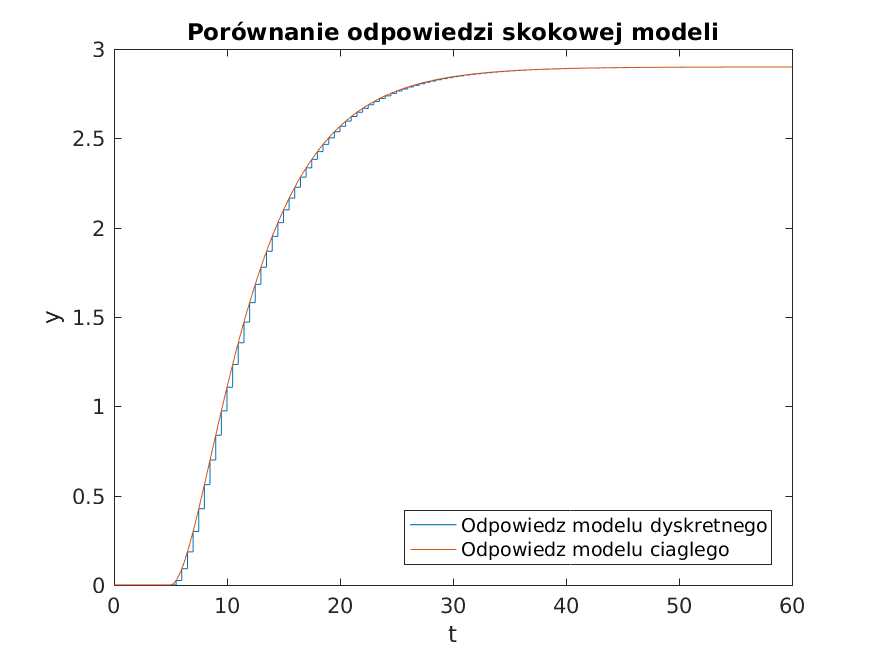
\includegraphics[width=0.7\linewidth]{z1_skok}
		\caption{}
		\label{fig:z1skok}
	\end{figure}
	
	\section{Równanie różnicowe}
	Dla transmitancji \[G(z)=z^{-10}\frac{0.0249z + 0.0225}{z^2 -1.7250z +0.7414} =\frac{0.0249z^{-11} + 0.0225z^{-12}}{1 -1.7250z^{-1} +0.7414z^{-2}}=\frac{Y(z)}{U(z)}\]
	Mamy:
	\[Y(z)(1 -1.7250z^{-1} +0.7414z^{-2}) = U(s)(0.0249z^{-11} + 0.0225z^{-12})\]
	Dlatego:
	\[y(k) = 1.7250y(k-1) - 0.7414y(k-2) + 0.0249y(k-11) + 0.0225y(k-12)\]

	\section{Regulator PID}
	Program znajduje się w pliku \textit{zadanie\_3.m}.\\
	Regulator ciągły dobrano, poprzez wyłączenie członów całkującego i różniczkującego regulatora (rys \ref{fig:z3kkciagly}). Uzyskano $K_k=0.817$ oraz $T_k = 21$. Dzięki temu dobrano $K_r=0.4902$, $T_i = 10.5$ oraz $T_d = 2.52$. Działanie układu z regulatorem jest widoczne na rysunku \ref{fig:z3pidciagly}.
	\begin{figure}
		\centering
		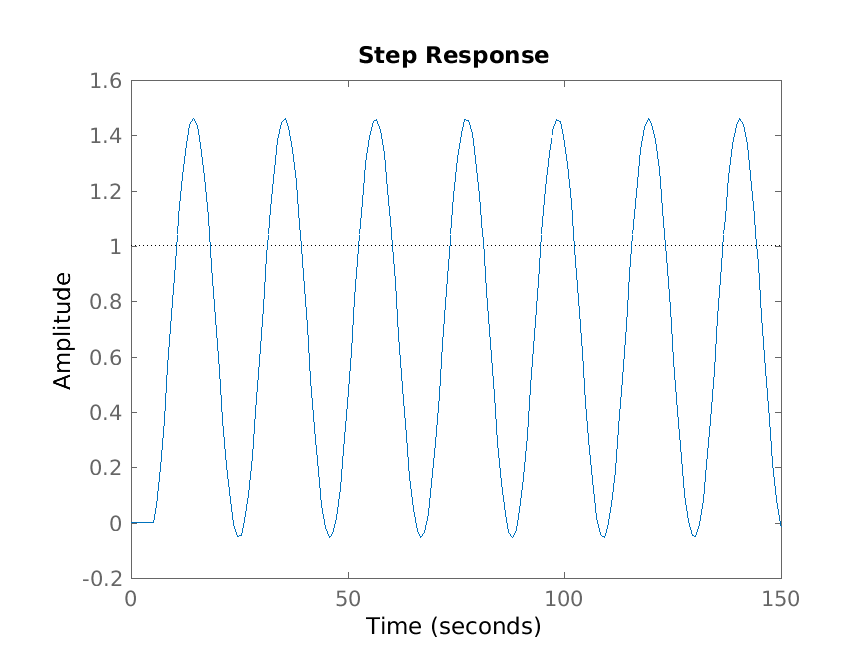
\includegraphics[width=0.7\linewidth]{z3_kk_ciagly}
		\caption{Układ przy wyłączonych członach różniczkującym i całkującym.}
		\label{fig:z3kkciagly}
	\end{figure}
	\begin{figure}
		\centering
		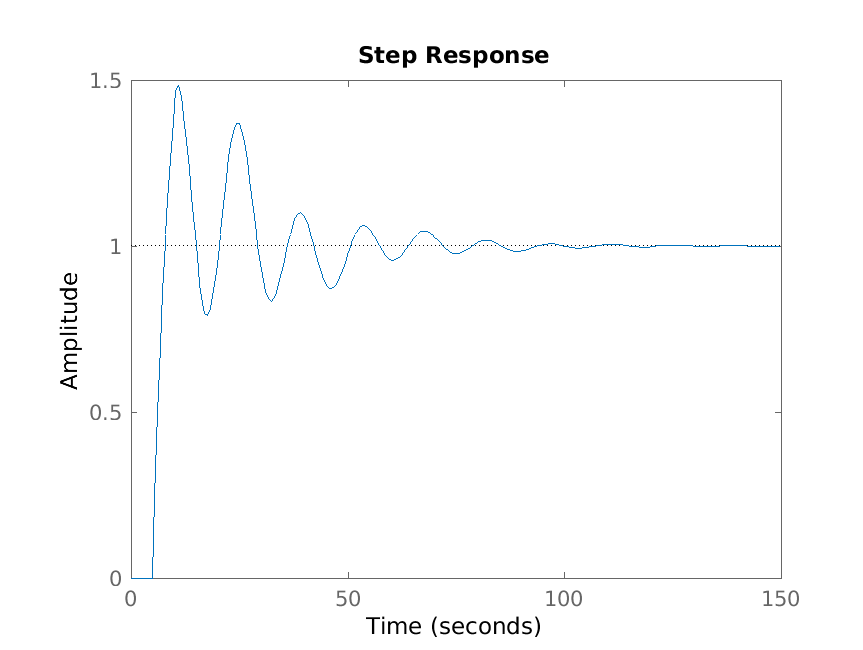
\includegraphics[width=0.7\linewidth]{z3_pid_ciagly}
		\caption{Układ z dobranym ciągłym regulatorem PID.}
		\label{fig:z3pidciagly}
	\end{figure}
	
	Regulator dyskretny ma postać:
	\[R(z)=\frac{U(z)}{E(z)}=\frac{r_2z^{-2} + r_1z^{-1} + r_0}{1 - z^{-1}}\]
	Przekształcając otrzymujemy:
	\[R(z) = \frac{(K_r + T_d) + (\frac{T_p}{T_i}-K_r-2T_d)z^{-1}+T_dz^{-2}}{1-z^{-1}}\]
	
	Transmitancję układu można też uzyskać z zależności:
	\[G(z) = \frac{z-1}{z}Z(\frac{G(s)}{s})\]
	
	Przyrównując obie postaci:
	\[r_2= T_d\]
	\[r_1=\frac{T_p}{T_i}-K_r-2T_d\]
	\[r_0=K_r + T_d\]
	
	więc:
	\[r_2= 2.52\]
	\[r_1= -5.4826\]
	\[r_0= 3.0102\]
	
	\section{Algorytm PID}
	Do symulacji wykorzystano obiekt opisany wcześniej transmitancją dyskretną.
	\subsection{Algorytm DMC}
	Implementacja znajduje się w pliku \textit{zadanie\_4\_dmc.m}.
	Rozwiązanie algorytmu DMC bazuje na zależności:
	\[\Delta u = (M^TM + \lambda I)^{-1}M^T(y^{zad}-y^k - M^P\Delta u^P)\]
	
	W celu wyznaczenia odpowiedzi skokowej zastosowano rozwiązania z zadania 1 (rysunek \ref{fig:z1skok}). Skorzystano z równań różnicowych z zadania 2.\\
	Przykładowa symulacja z parametrami:
	\begin{itemize}
		\item horyzont predykcji $N=60$
		\item horyzont dynamiki $D = 60$
		\item horyzont sterowania $N_u = 3$
		\item wskaźnik jakości $\lambda = 10$
	\end{itemize}
	zaprezentowana jest na rysunku \ref{fig:z4}.
	\begin{figure}
		\centering
		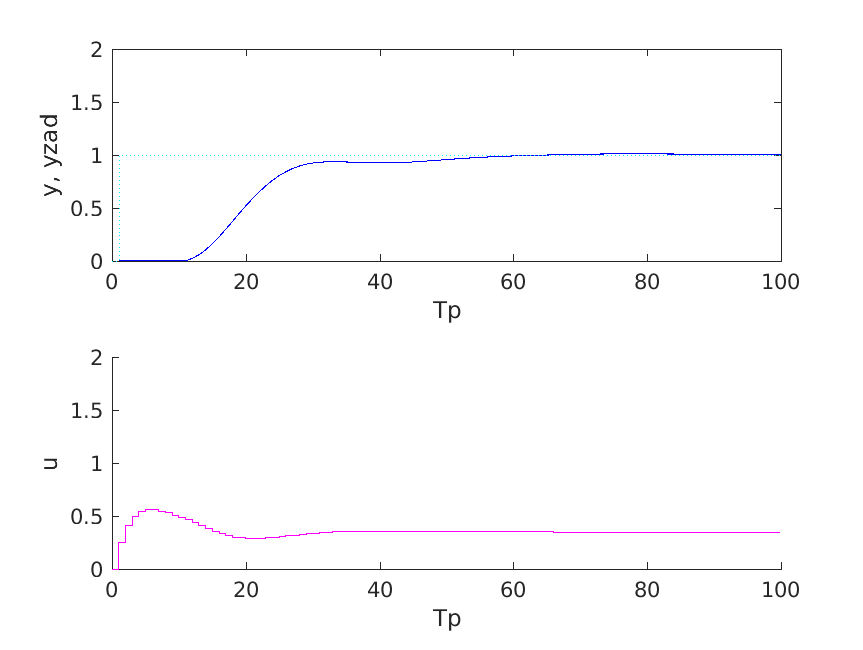
\includegraphics[width=0.7\linewidth]{z4}
		\caption{Przykładowa symulacja algorytmu DMC.}
		\label{fig:z4}
	\end{figure}
	
	\section{Dobór parametrów algorytmu DMC}
	\subsection{Horyzont dynamiki}
	Sygnał odpowiedzi skokowej stabilizuje się po 50 s. Dlatego $D = 50/T_p = 100$. Założono $\lambda = 1$. Symulację przedstawia rysunek \ref{fig:z5_100_100_100_1}. 
	\begin{figure}
		\centering
		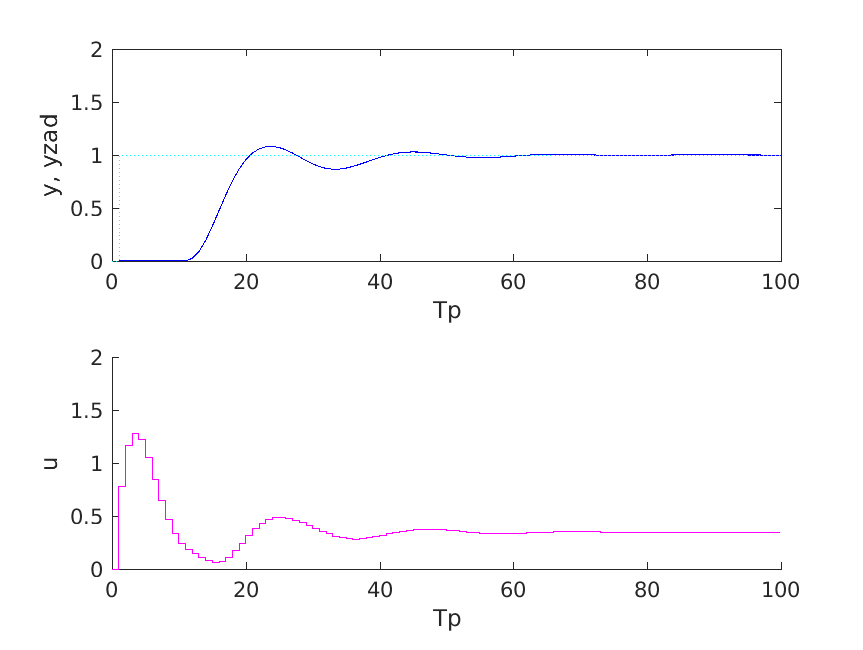
\includegraphics[width=0.7\linewidth]{z5_100_100_100_1.png}
		\caption{Symulacja DMC dla parametrów $N=Nu=D=100, \lambda = 1$}
		\label{fig:z5_100_100_100_1}
	\end{figure}
	\subsection{Horyzont predykcji}
	Wybrano $N=60$ ponieważ jest to najmniejsza z wartości, dla których algorytm nie zachowywał się gorzej, niż w przypadku z podpunktu a). Symulację przedstawia rysunek 
	\begin{figure}
		\centering
		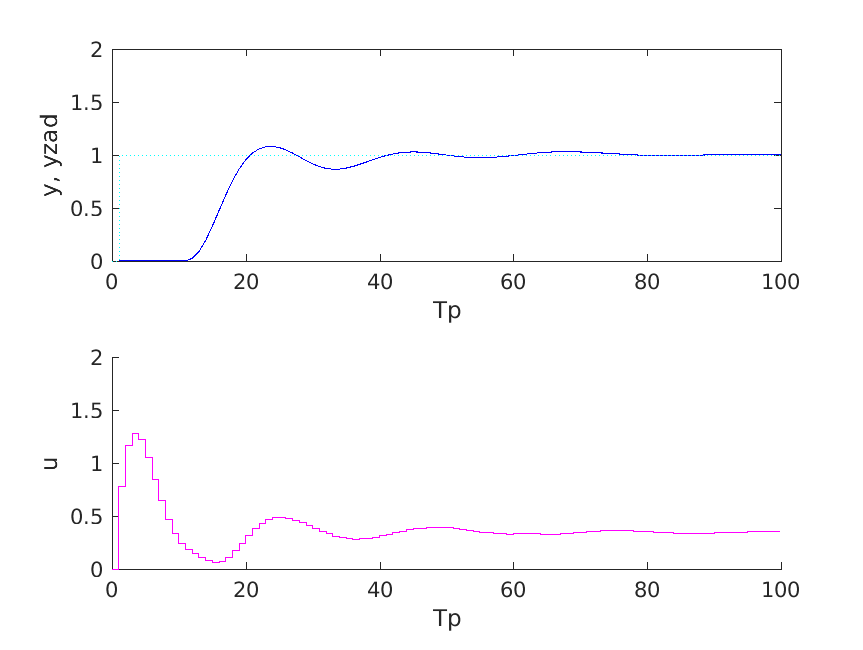
\includegraphics[width=0.7\linewidth]{z5_60_60_60_1.png}
		\caption{Symulacja DMC dla parametrów $N=Nu=60, \lambda = 1$}
		\label{fig:z5_60_60_60_1}
	\end{figure}
	\subsection{Horyzont sterowania}
	Przeprowadzono szereg symulacji zaprezentowanych na rysunkach \ref{fig:z5_60_60_1_1}, \ref{fig:z5_60_60_2_1}, \ref{fig:z5_60_60_3_1}, \ref{fig:z5_60_60_4_1}, \ref{fig:z5_60_60_5_1}, \ref{fig:z5_60_60_10_1}, \ref{fig:z5_60_60_20_1}, \ref{fig:z5_60_60_30_1}, \ref{fig:z5_60_60_40_1}, \ref{fig:z5_60_60_50_1} i 
	\ref{fig:z5_60_60_60_1}. Okazuje się, że dla $N_u > 10 $ symulacja zachowuje się dość podobnie. Ze wzrostem parametru zwiększają się oscylacje. Nie ma więc sensu stosowanie większych horyzontów sterowania. Dla parametru $N_u = 1$ nie występuje przeregulowanie, co w niektórych zastosowaniach może być dużą zaletą.
	Według autora najlepszym kompromisem pomiędzy szybkością regulacji, maksymalną różnicą skoków sterowania, przeregulowaniem oraz złożonością algorytmu jest $N_u = 10$.
	\begin{figure}
		\centering
		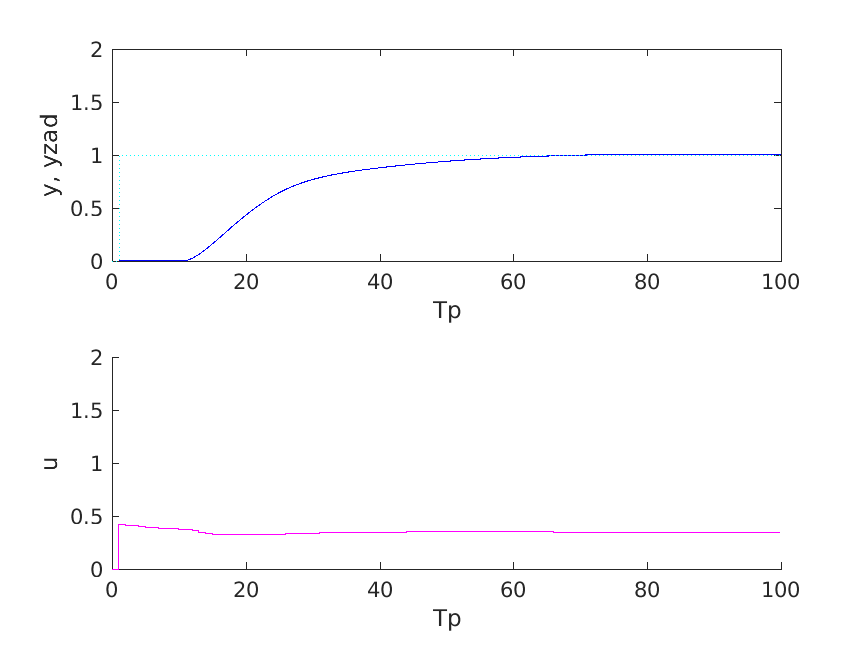
\includegraphics[width=0.7\linewidth]{z5_60_60_1_1.png}
		\caption{Symulacja DMC dla parametrów $N=60, Nu = 1, \lambda = 1$}
		\label{fig:z5_60_60_1_1}
	\end{figure}\begin{figure}
	\centering
	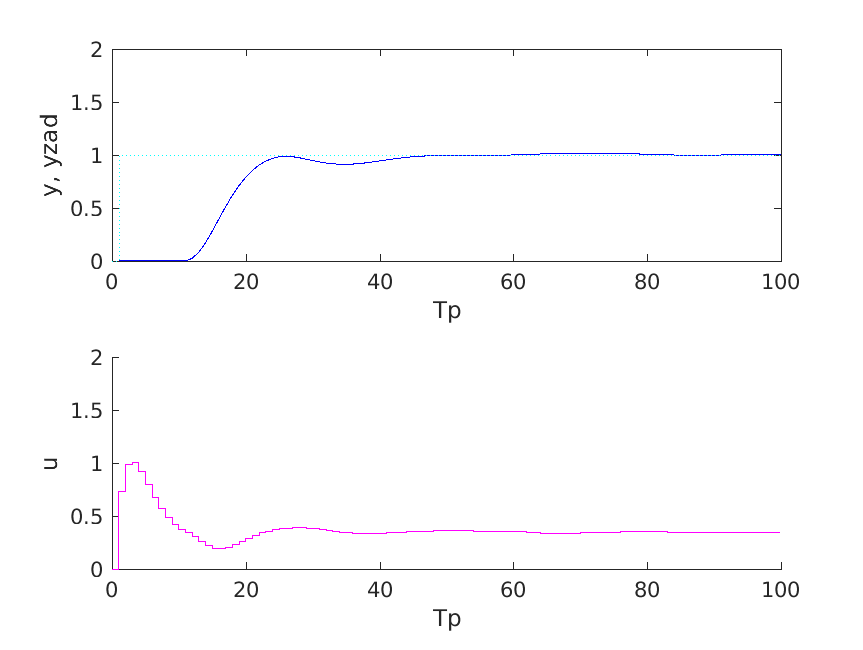
\includegraphics[width=0.7\linewidth]{z5_60_60_2_1.png}
	\caption{Symulacja DMC dla parametrów $N=60, Nu = 2, \lambda = 2$}
	\label{fig:z5_60_60_2_1}
\end{figure}\begin{figure}
\centering
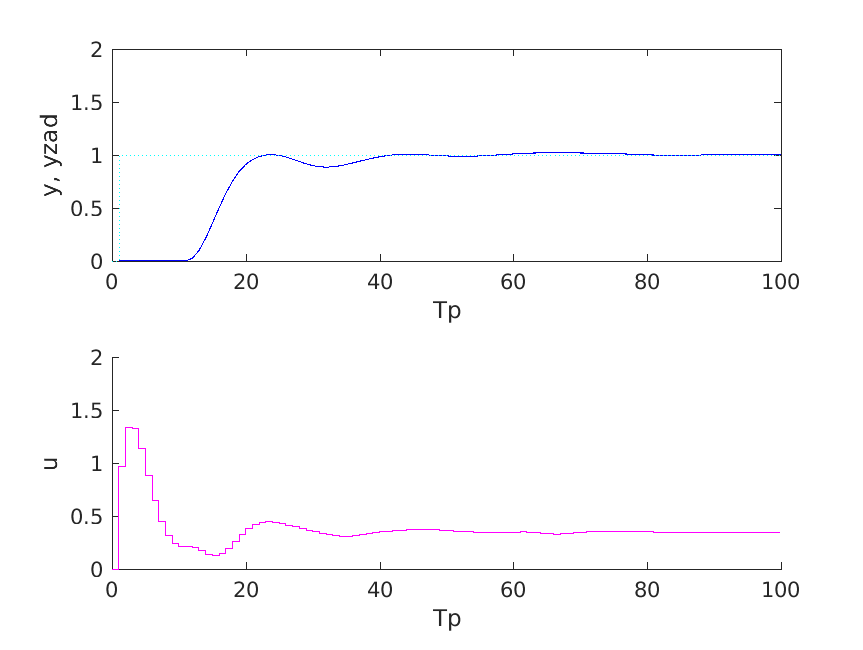
\includegraphics[width=0.7\linewidth]{z5_60_60_3_1.png}
\caption{Symulacja DMC dla parametrów $N=60, Nu = 3, \lambda = 1$}
\label{fig:z5_60_60_3_1}
\end{figure}\begin{figure}
\centering
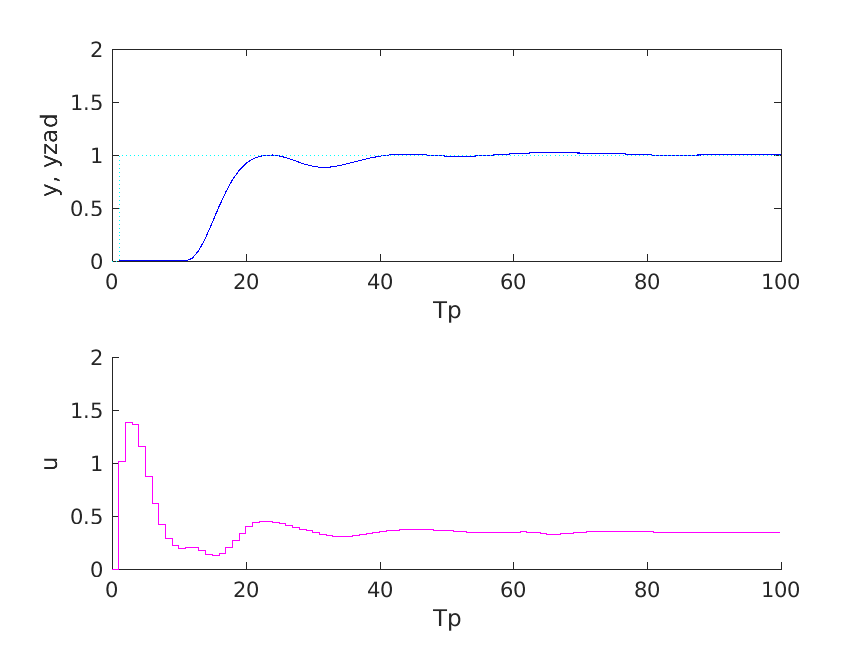
\includegraphics[width=0.7\linewidth]{z5_60_60_4_1.png}
\caption{Symulacja DMC dla parametrów $N=60, Nu = 4, \lambda = 1$}
\label{fig:z5_60_60_4_1}
\end{figure}\begin{figure}
\centering
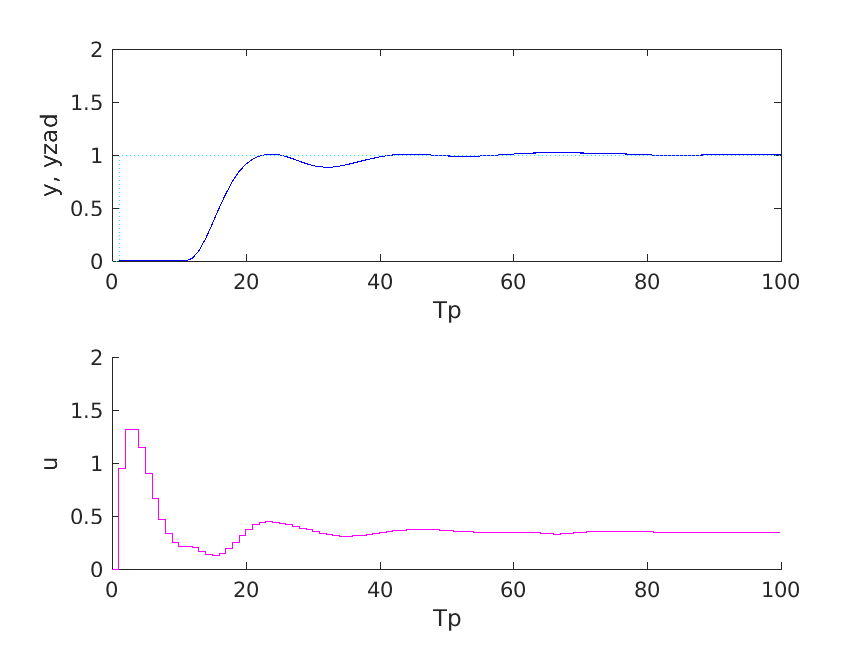
\includegraphics[width=0.7\linewidth]{z5_60_60_5_1.png}
\caption{Symulacja DMC dla parametrów $N=60, Nu = 5, \lambda = 1$}
\label{fig:z5_60_60_5_1}
\end{figure}
	\begin{figure}
		\centering
		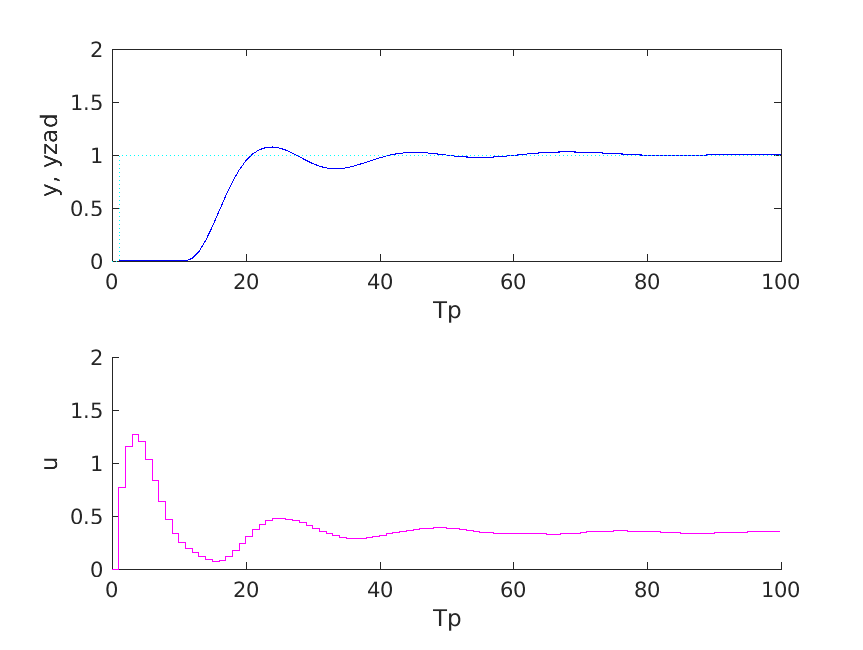
\includegraphics[width=0.7\linewidth]{z5_60_60_10_1.png}
		\caption{Symulacja DMC dla parametrów $N=60, Nu = 10, \lambda = 1$}
		\label{fig:z5_60_60_10_1}
	\end{figure}
	\begin{figure}
		\centering
		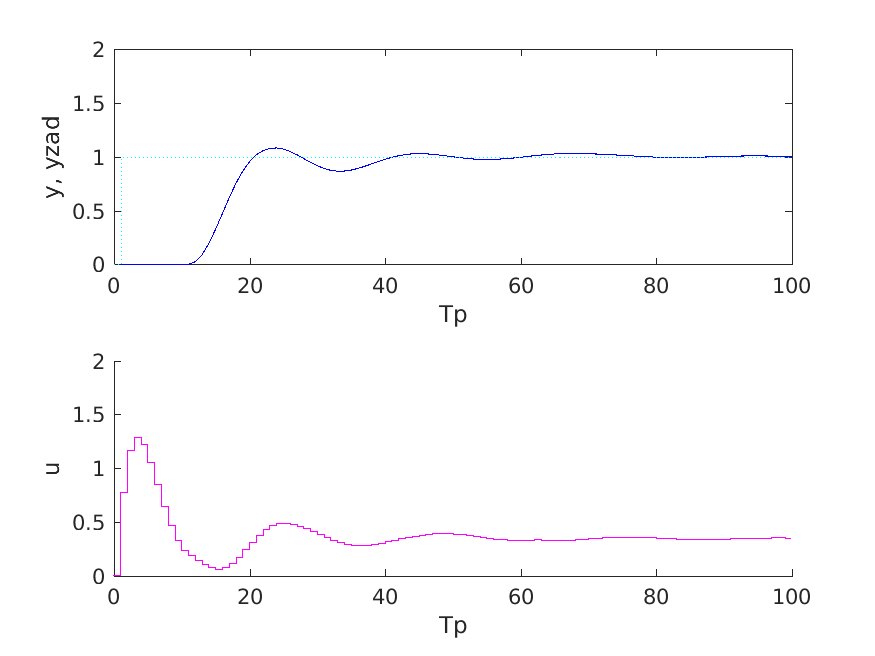
\includegraphics[width=0.7\linewidth]{z5_60_60_20_1.png}
		\caption{Symulacja DMC dla parametrów $N=60, Nu = 20, \lambda = 1$}
		\label{fig:z5_60_60_20_1}
	\end{figure}\begin{figure}
	\centering
	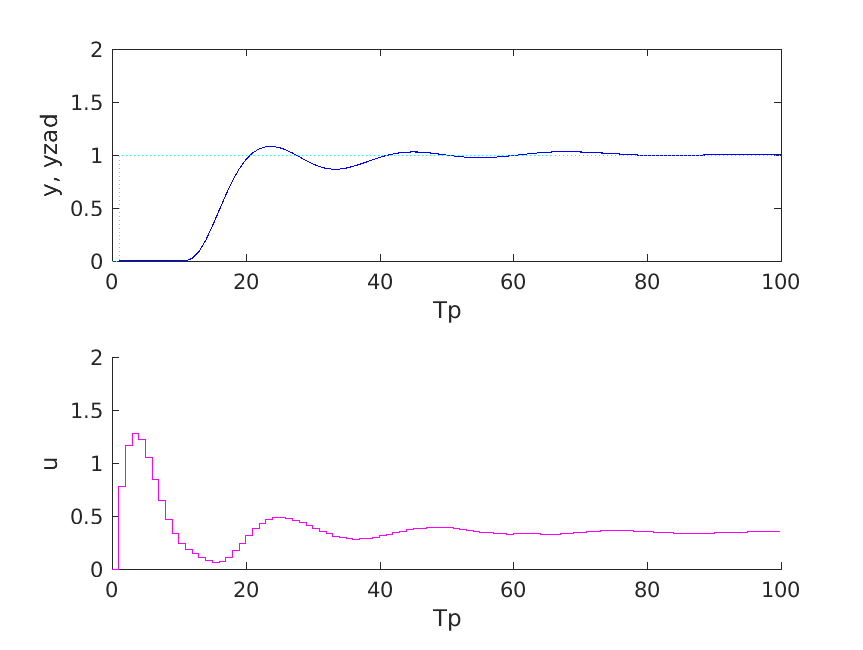
\includegraphics[width=0.7\linewidth]{z5_60_60_30_1.png}
	\caption{Symulacja DMC dla parametrów $N=60, Nu = 30, \lambda = 1$}
	\label{fig:z5_60_60_30_1}
\end{figure}\begin{figure}
\centering
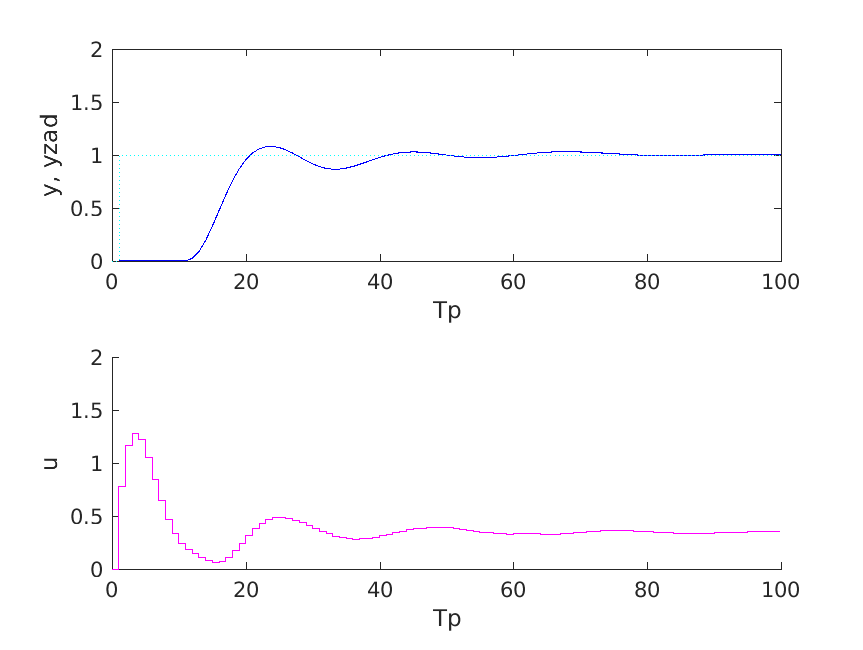
\includegraphics[width=0.7\linewidth]{z5_60_60_40_1.png}
\caption{Symulacja DMC dla parametrów $N=60, Nu = 40, \lambda = 1$}
\label{fig:z5_60_60_40_1}
\end{figure}\begin{figure}
\centering
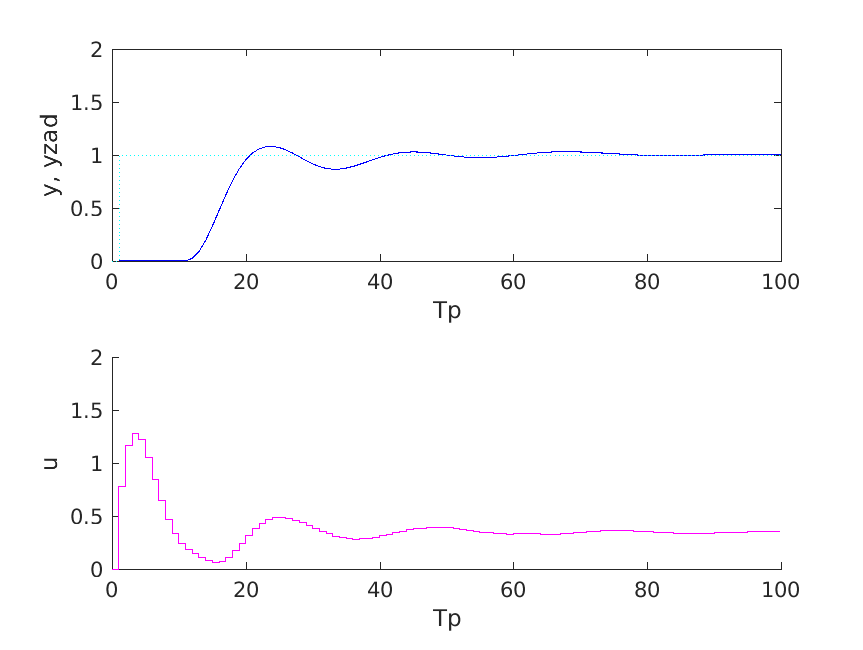
\includegraphics[width=0.7\linewidth]{z5_60_60_50_1.png}
\caption{Symulacja DMC dla parametrów $N=60, Nu = 50, \lambda = 1$}
\label{fig:z5_60_60_50_1}
\end{figure}

\subsection{Współczynnik $\lambda$}
Przeprowadzono symulacje zaprezentowane na rysunkach \ref{fig:z5_60_60_10_1}, \ref{fig:z5_60_60_10_5}, \ref{fig:z5_60_60_10_10}, \ref{fig:z5_60_60_10_20}, \ref{fig:z5_60_60_10_40} i \ref{fig:z5_60_60_10_60}. Według autora nalepszym kompromisem pomiędzy postacią sygnału wyjściowego i szybkością jest $\lambda = 5$. 
\begin{figure}
	\centering
	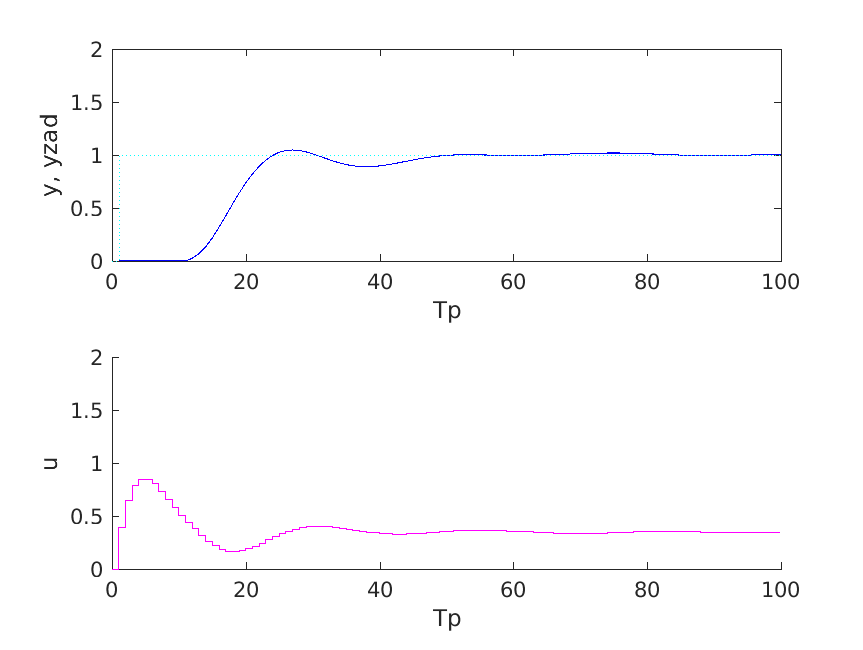
\includegraphics[width=0.7\linewidth]{z5_60_60_10_5.png}
	\caption{Symulacja DMC dla parametrów $N=60, Nu = 10, \lambda = 5$}
	\label{fig:z5_60_60_10_5}
\end{figure}
\begin{figure}
	\centering
	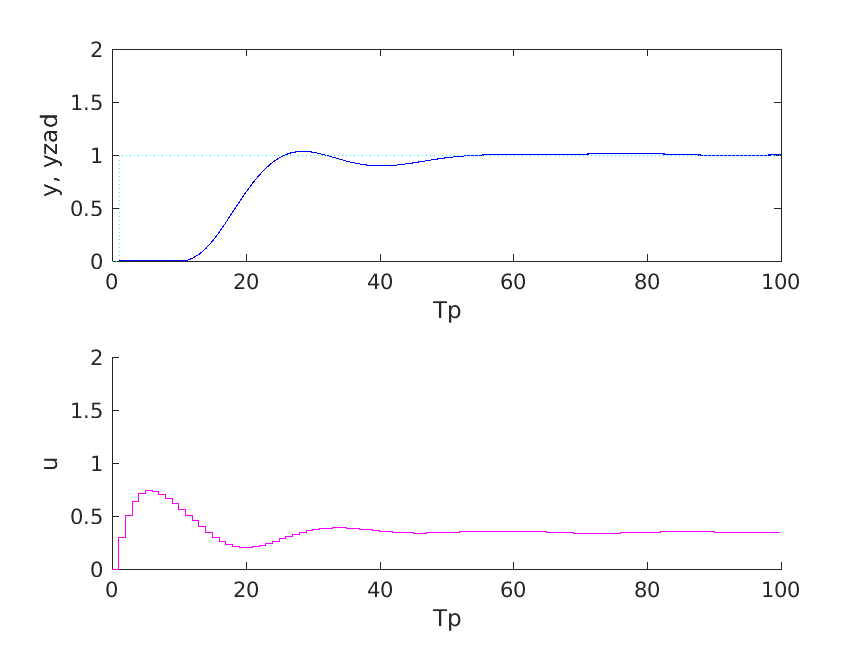
\includegraphics[width=0.7\linewidth]{z5_60_60_10_10.png}
	\caption{Symulacja DMC dla parametrów $N=60, Nu = 10, \lambda = 10$}
	\label{fig:z5_60_60_10_10}
\end{figure}
\begin{figure}
	\centering
	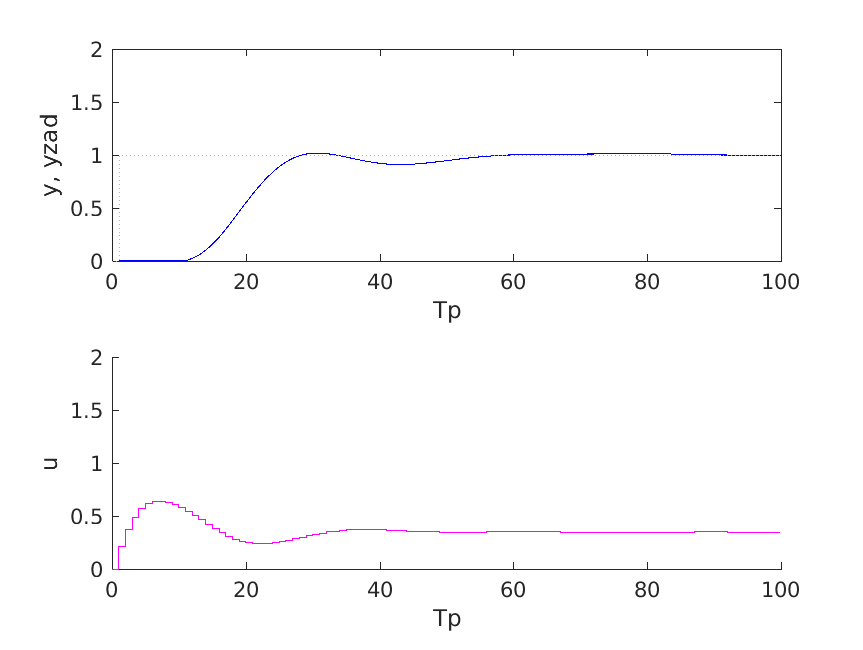
\includegraphics[width=0.7\linewidth]{z5_60_60_10_20.png}
	\caption{Symulacja DMC dla parametrów $N=60, Nu = 10, \lambda = 20$}
	\label{fig:z5_60_60_10_20}
\end{figure}
\begin{figure}
	\centering
	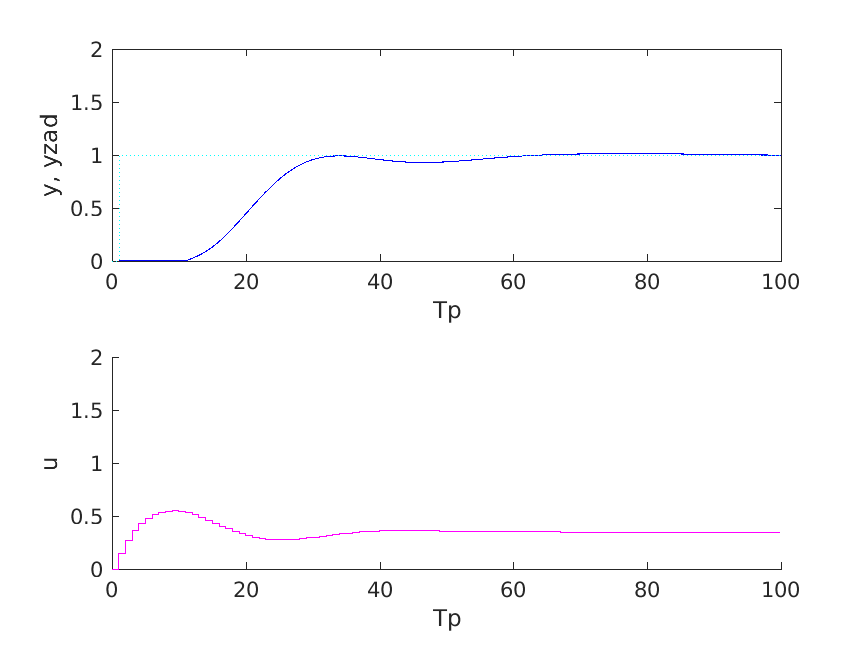
\includegraphics[width=0.7\linewidth]{z5_60_60_10_40.png}
	\caption{Symulacja DMC dla parametrów $N=60, Nu = 10, \lambda = 40$}
	\label{fig:z5_60_60_10_40}
\end{figure}
\begin{figure}
	\centering
	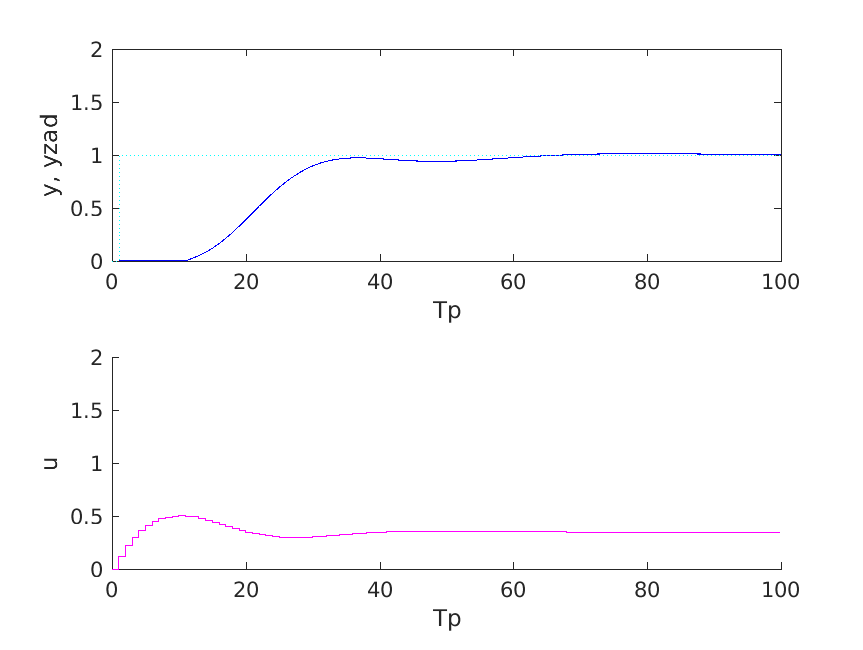
\includegraphics[width=0.7\linewidth]{z5_60_60_10_60.png}
	\caption{Symulacja DMC dla parametrów $N=60, Nu = 10, \lambda = 60$}
	\label{fig:z5_60_60_10_60}
\end{figure}
\section{Porównanie algorytmów PID i DMC}
	
\end{document}